% La plantilla usada es la siguiente por si acaso le guste la plantilla profe
%%%%%%%%%%%%%%%%%%%%%%%%%%%%%%%%%%%%%%%%%
% ELEE	3720 Electromechanical Energy Conversion: Report template
% By Ratheesh Ravindran
%%%%%%%%%%%%%%%%%%%%%%%%%%%%%%%%%%%%%%%%%
\documentclass[12pt]{article}
\usepackage[spanish]{babel}
\usepackage[utf8]{inputenc}
\usepackage{amsmath}
\usepackage{graphicx}
\graphicspath{{Images/}}
\usepackage[colorinlistoftodos]{todonotes}
\usepackage{hyperref}
\usepackage{fancyhdr}
\usepackage{listings}%para poder mostrar codigo mas facil
\pagestyle{fancy}

%%DEFINIMOS LOS COLORES PARA JAVA
\definecolor{pblue}{rgb}{0.13,0.13,1}
\definecolor{pgreen}{rgb}{0,0.5,0}
\definecolor{pred}{rgb}{0.9,0,0}
\definecolor{pgrey}{rgb}{0.46,0.45,0.48}

%DEFINIMOS EL FORMATO DEL CODIGO DE JAVA
\lstset{language=Java,
  showspaces=false,
  showtabs=false,
  breaklines=true,
  showstringspaces=false,
  breakatwhitespace=true,
  commentstyle=\color{pgreen},
  keywordstyle=\color{pblue},
  stringstyle=\color{pred},
  basicstyle=\ttfamily,
  moredelim=[il][\textcolor{pgrey}],
  moredelim=[is][\textcolor{pgrey}]{\%\%}{\%\%}
}
%---------------------------------------------------------
%----------VARIABELES QUE SERAN UTILIZADAS DESPUES--------
%---------------------------------------------------------

\newcommand{\documentTitle}{Proyecto Final POO}
\newcommand{\Creador}{Carlos Daniel Hernandez Chauteco}
\newcommand{\profesor}{Ing. Guadalupe Lizeth Parrales Romay}

%---------------------------------------------------------

\begin{document}
\begin{titlepage}
\newcommand{\HRule}{\rule{\linewidth}{0.1mm}} 
\center %esta linea ayuda a centrar todo en la pantalla
%-----------------------------------------------------------
%----------------ESTA PARTE ES PARA LOS ENCABEZADOS--------
%----------------------------------------------------------

\lhead{\documentTitle}

%------------------------------------------------------------
%----------------ESTA PARTE ES PARA EL HEADER-----------
%-----------------------------------------------------------
%unam logos

\includegraphics{escudounam_negro.jpg} \hfill 
\includegraphics{fiEscudo.jpg}\\[1cm]
%end unam logos

\textsc{\Large Programación Orientada a Objetos}\\[0.5cm]
\textsc{\large Proyecto Final}\\[0.5cm]
{\large \today}\\[1cm]%FECHA DE COMPILACION
%---------------------------------------------------------------------------------
% SECCION PARA EL TITULO
%---------------------------------------------------------------------------------

\HRule \\[0.4cm]
{ \huge \bfseries \documentTitle}\\[0.1cm]
\HRule \\[1.5cm]
 
%---------------------------------------------------------------------------------
%	SECCION DE AUTORES
%---------------------------------------------------------------------------------
%--Aqui estan los nombres de los integrantes
\begin{minipage}{0.4\textwidth}
\begin{flushleft} \large
\emph{Alumno}\\
\textsc{\Creador} 
\end{flushleft}


\begin{flushleft} \large

\emph{Profesora}\\
\textsc{\profesor} % aqui van los nombres
\end{flushleft}

\end{minipage}

\vfill
\hfill
\newline
\begin{quote}
    \hfill
    
\includegraphics{by-nc-sa.png}
\end{quote}

\vfill % Deja un espacio en blanco para que no haya mas en la pagina

\end{titlepage}
%\tableofcontents         %Lista de contenido
\newpage

% AQUI EMPIEZA EL CUERPOD DEL DOCUMENTO

%Aqui van las secciones del documento
\section{Justificación Del Proyecto}
\subsection{Resumen}
El proyecto nace de una pequeña idea que tenia la cual es hacer una aplicación que busque entre muchas personas con tu mismos gustos con demás personas  así nació la idea de la aplicación aunque al principio se suponía que era una aplicación de citas tengo pensado que si la llego a escalar a mas esta puede ser una aplicación para conocer gente con los mismos gustos y que no solo se limite a citas como en un principio se pensaba el principal problema para esta aplicación fue el backend que era inexistente y no sabia en concreto como lo iba hacer hasta que recordé el backend de Firebase que funciona como plataforma como servicio el cual me proporciona un backend con ciertas restricciones para las cuentas gratuitas pero que me soluciona el problema rápido y también a futuro cuando aprenda alguna tecnología de backend podria hacer el servidor.

\section{Descripción}
La aplicación esta hecha en java con el entorno de desarrollo de android studio para facilitar el desarrollo de la aplicación esta también esta escrita con mucho código XML que es el que define la interfaz gráfica del las aplicaciones con android la aplicación por el momento solo ha sido hecha para android así que solo esta en esta plataforma posiblemente se desarrolle su contra parte en ios

\section{Código Fuente}
%\lstinputlisting{JavaCode/ChatActivity.java}
Como la aplicación contiene mucho código decidí que este apartado solo contuviera el código de las clases que me parecieran importantes que son las mas 'importantes' para la aplicación a MainActitity no lo pogo por que no cabe en el documento  
\newpage
Login Activity:
\lstinputlisting{JavaCode/LoginActivity.java}
\newpage
Chat Activity:
\lstinputlisting{JavaCode/ChatActivity.java}
\newpage
login Activity:
\lstinputlisting{JavaCode/LoginActivity.java}
\newpage
Profile Activity:
\lstinputlisting{JavaCode/ProfileActivity.java}
\newpage
Por supuesto los modelos de datos que utilize para apliacion son super importantes

Person:
\lstinputlisting{JavaCode/Person.java}
\newpage
Message:
\lstinputlisting{JavaCode/Message.java}

\section{Diagramas UML}
Diagrama de caso de uso de la aplicación:

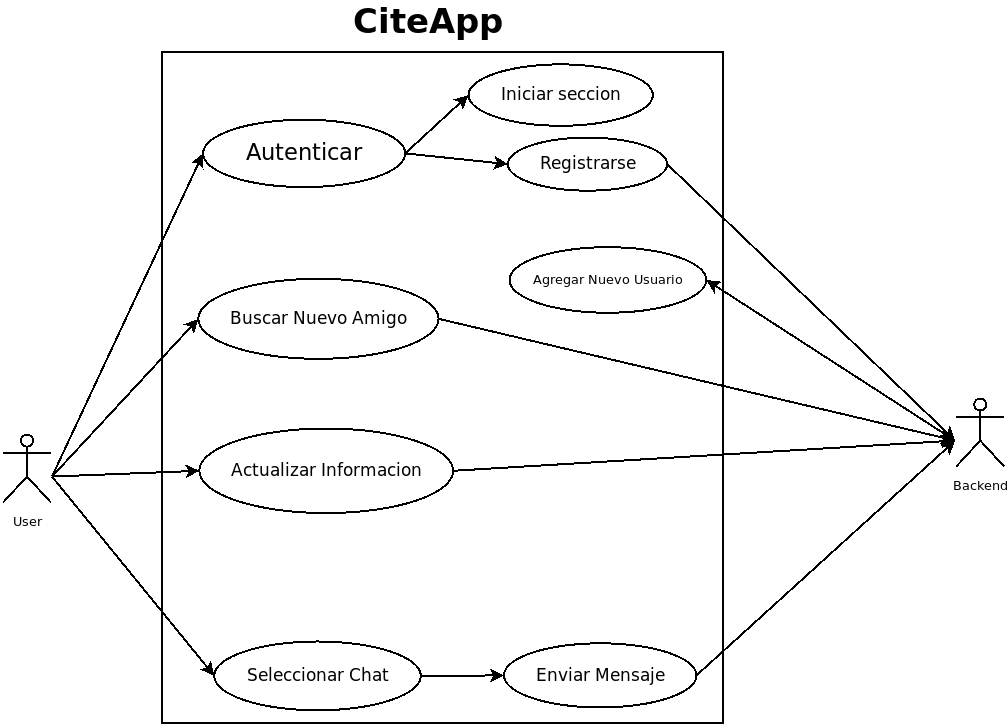
\includegraphics[width=13cm]{Images/UML/CasoUso.png}

Diagrama de Objetos:

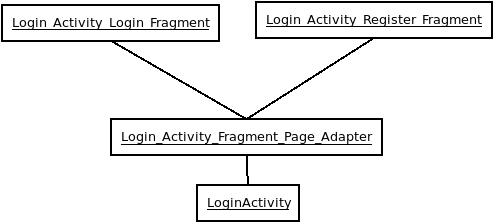
\includegraphics[width=13cm]{Images/UML/LoginActivityDiagramObject.png}

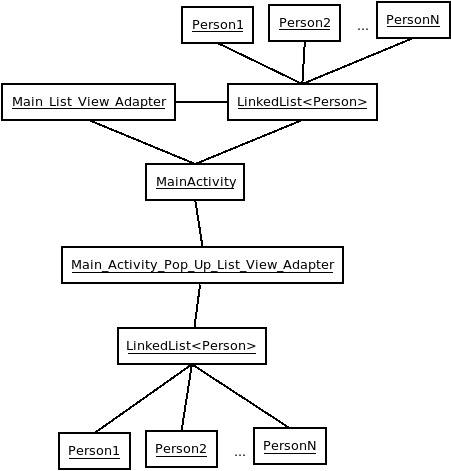
\includegraphics[width=13cm]{Images/UML/MainActivityDiagramObject.png}

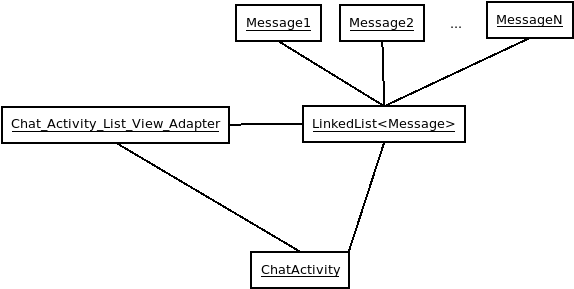
\includegraphics[width=13cm]{Images/UML/ChatActivityDiagramObject.png}

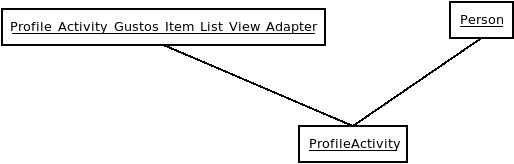
\includegraphics[width=13cm]{Images/UML/ProfileActivityDiagramObject.png}

Diagrama de clases:

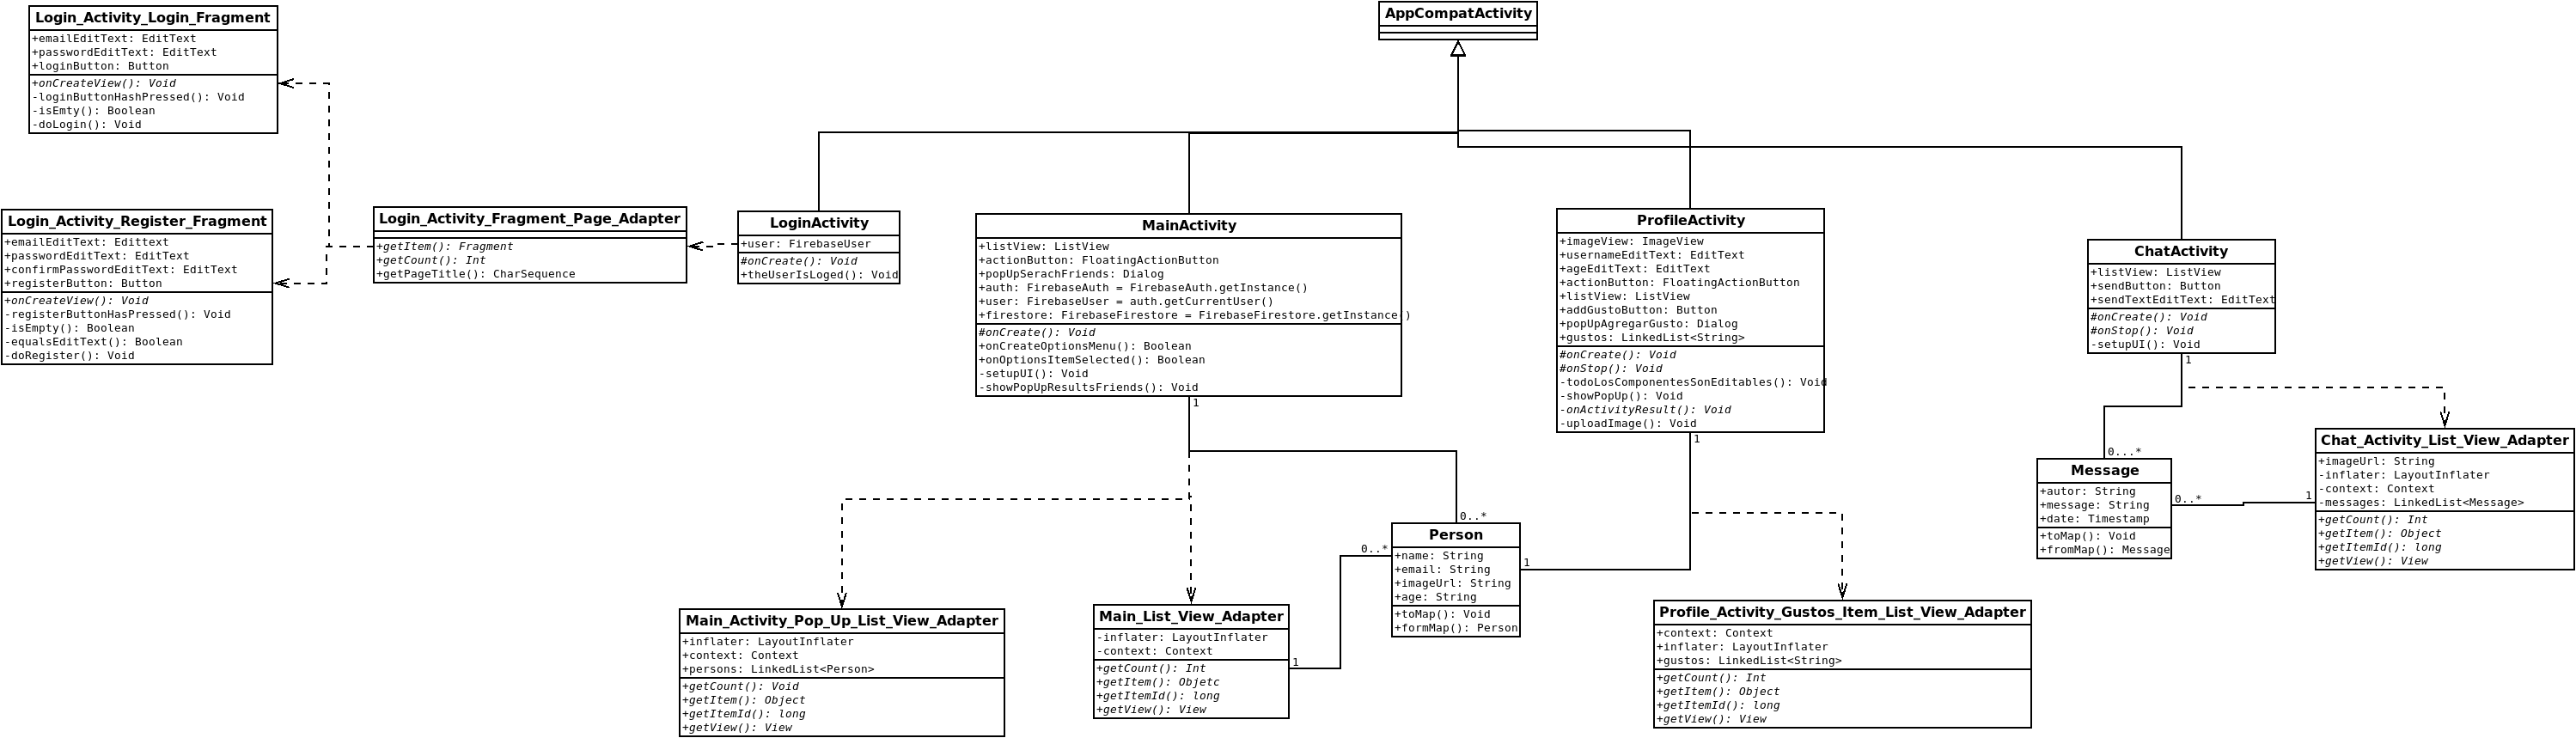
\includegraphics[angle=90,scale=0.25]{Images/UML/Clase.png}

Diagrama de Componentes:

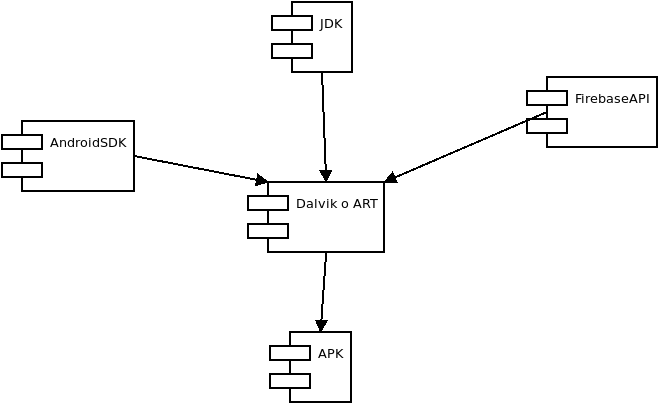
\includegraphics[width=13cm]{Images/UML/Componentes.png}

Diagrama de Despliegue:

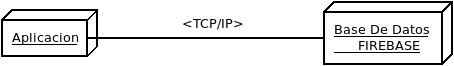
\includegraphics[width=13cm]{Images/UML/Despliegue.png}

\section{Capturas de Pantalla}
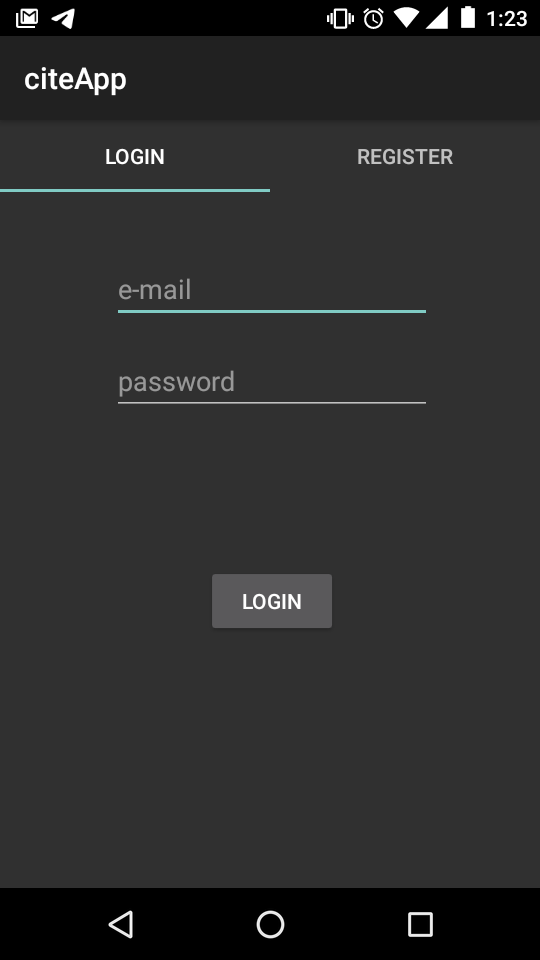
\includegraphics[width=12cm]{Images/Capturas/1.png}

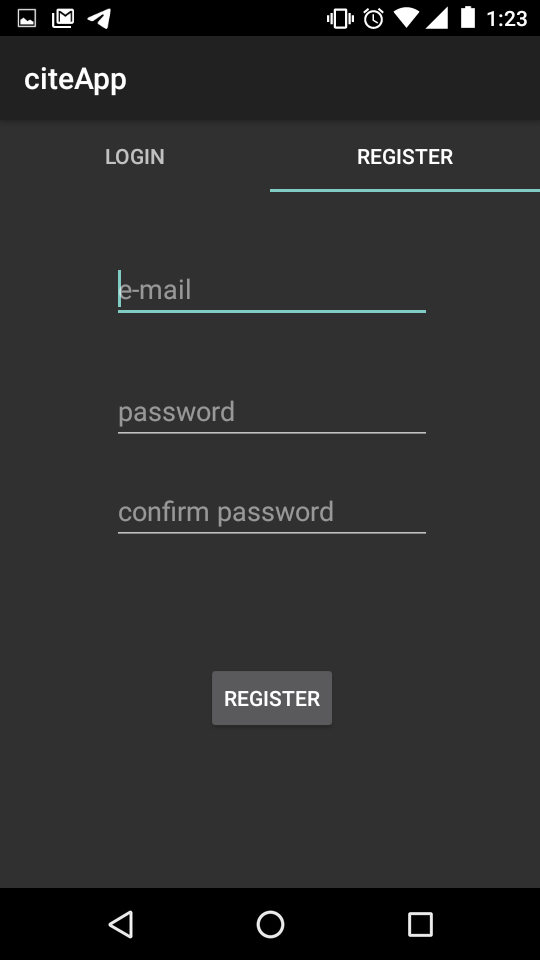
\includegraphics[width=12cm]{Images/Capturas/2.png}

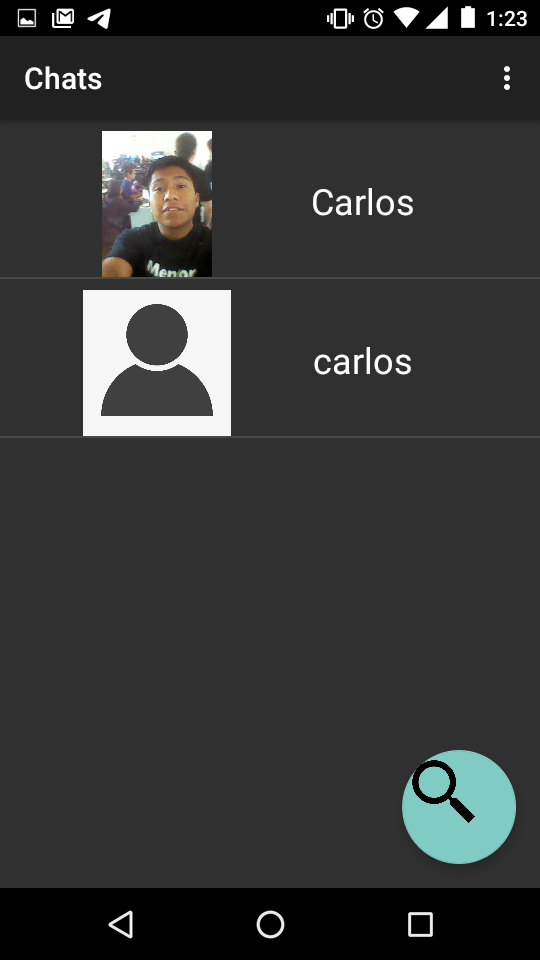
\includegraphics[width=12cm]{Images/Capturas/3.png}

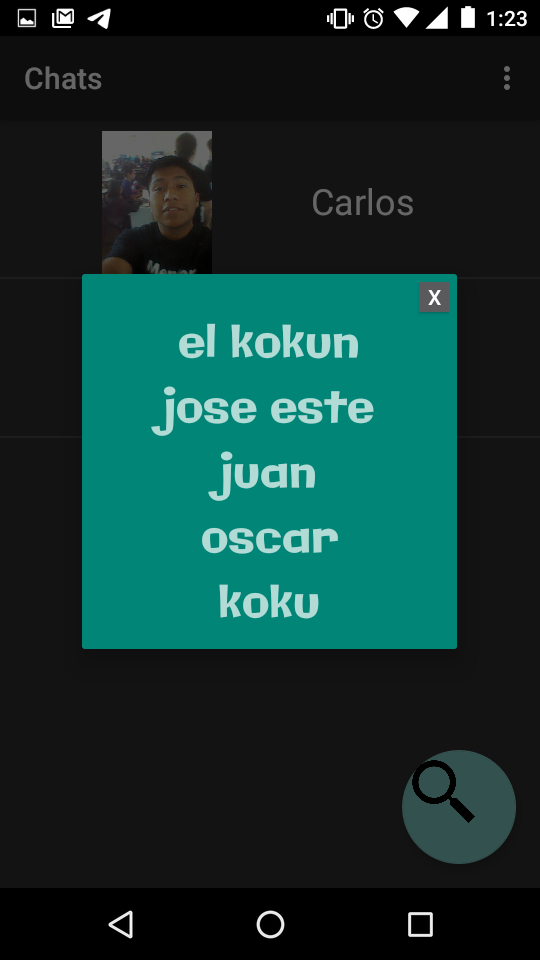
\includegraphics[width=12cm]{Images/Capturas/4.png}

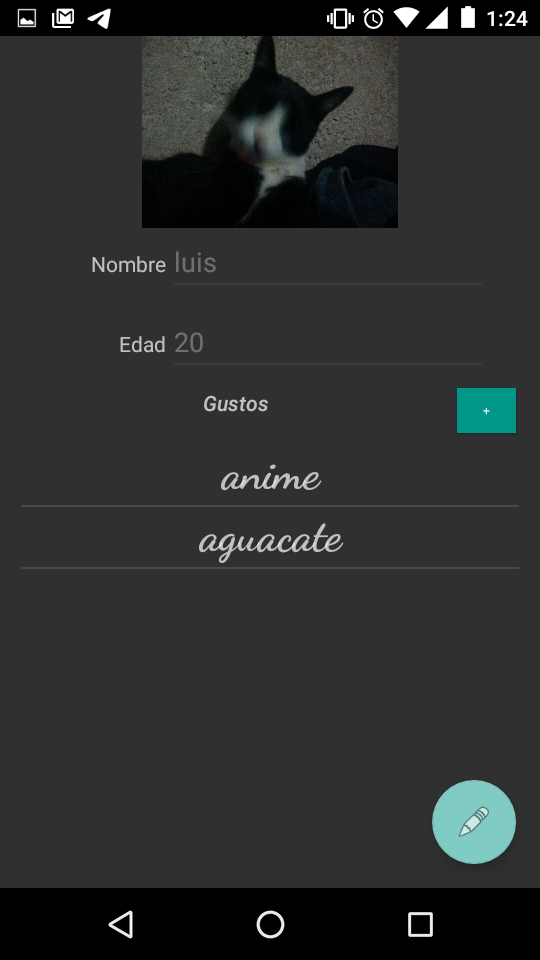
\includegraphics[width=12cm]{Images/Capturas/5.png}

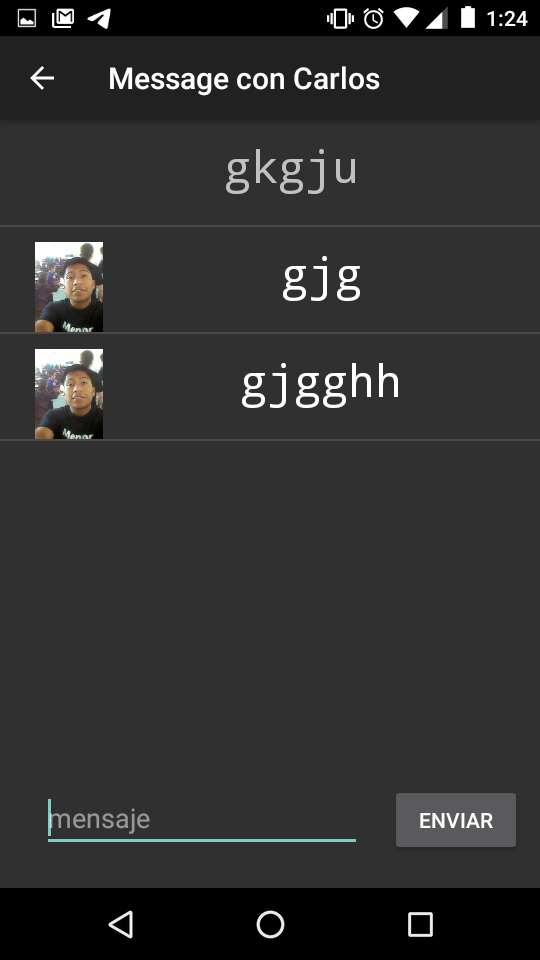
\includegraphics[width=12cm]{Images/Capturas/6.png}


%BIBLIOGRAFIA CITADO EN el formato de ACM 
%Nota: si el equipo lo quiere lo podemos cambiar a appa o cualquier otro que ellos quieran

%\bibliographystyle{acm}
%\bibliography{bibliografia}



\end{document}